\chapter{Model}
Należy wpierw stworzyć doskonały model kinematyczny, aby móc porównać z nim stworzony model dynamiczny, oraz fizyczną platformę.
Dzięki temu można łatwo oszacować jak bardzo błędy symulacji, oraz błędy niedoskonałości fizycznego modelu odstają od matematycznych wyliczeń.

Dodatkowo stworzenie platformy kinematycznej pozwalało na porównanie szybkie odrzucanie niedziałających implementacji modelu kinematycznego.
\begin{figure}[H]
\centering
 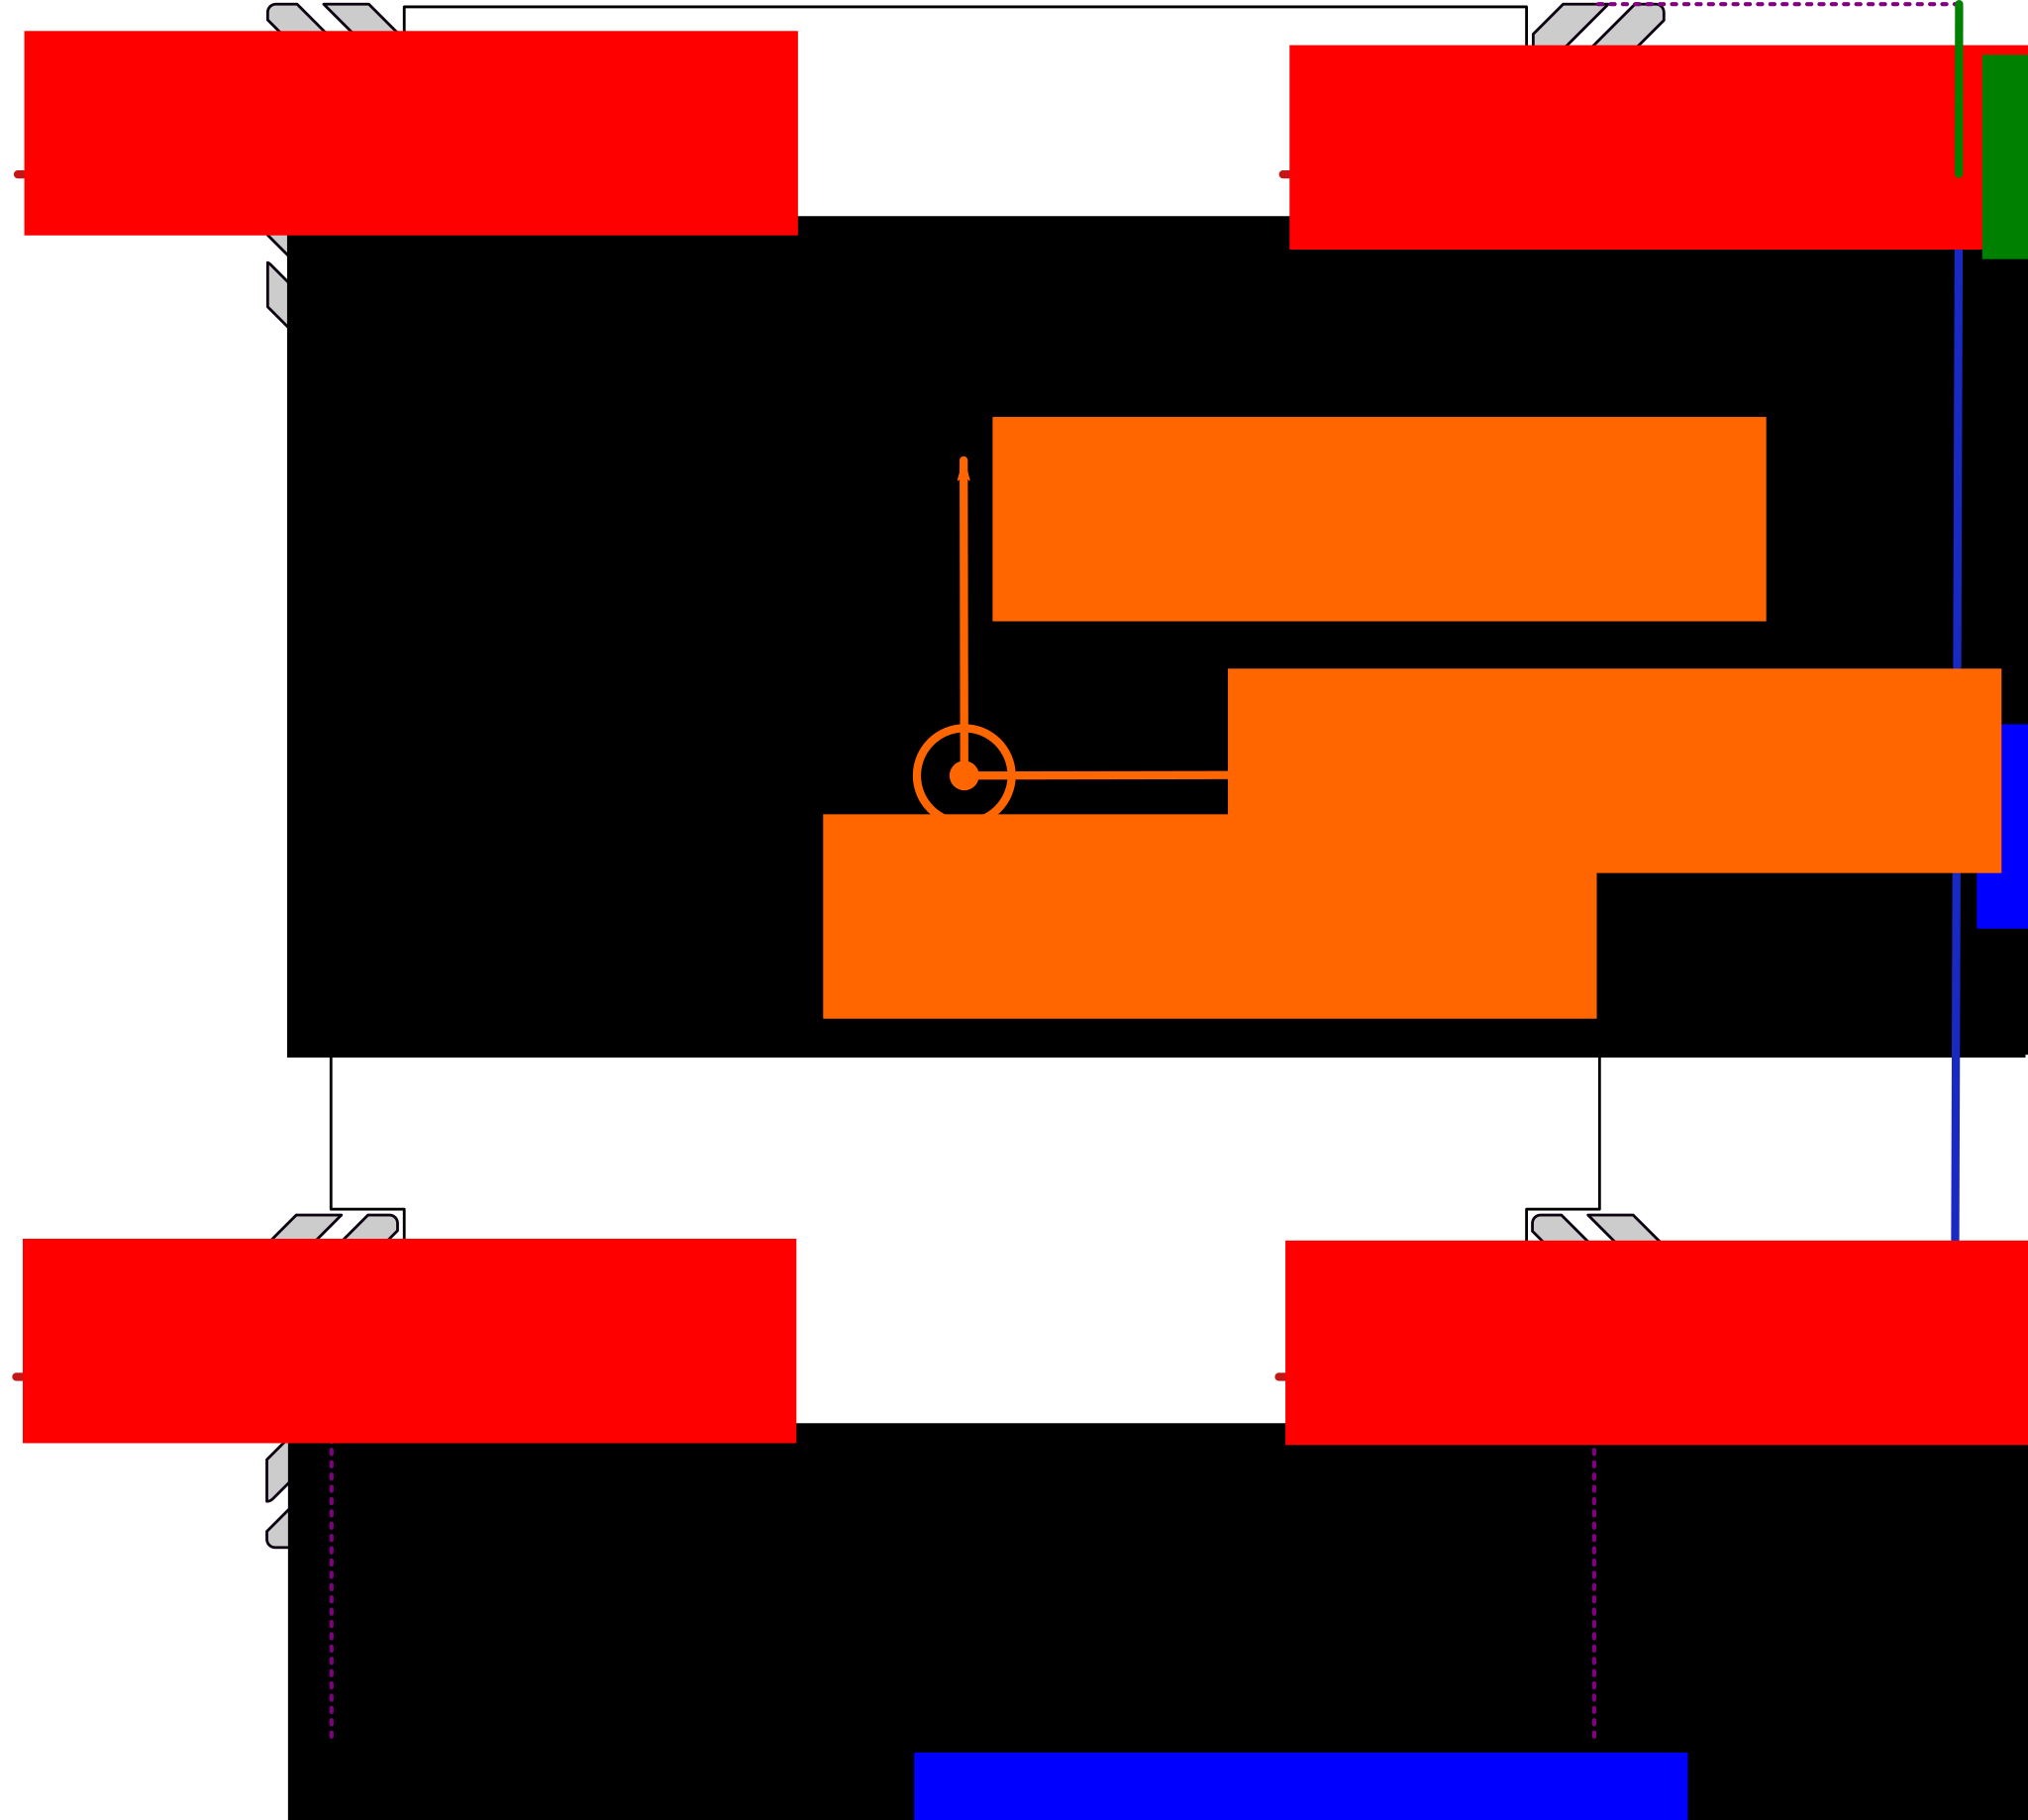
\includegraphics[width=0.8\textwidth]{graphics/base_dims.pdf}
\caption{Wielkości używane we wzorach.}
\end{figure} 
\begin{tabular}{l c l}
Oznaczenie & Wartość & Opis \\
\hline
$r$ & 0,1 m & Promień koła w najszerszym miejscu na środku. \\
$a$ & 0,76 m & Szerokość platformy między środkami kół tej samej osi. \\
$b$ & 0,72 m & Długość platformy między środkami kół tego samego boku. \\
$\omega_i$ & & Prędkość kątowa każdego z kół. \\
$V_x$ & & Prędkość transwersalna w osi X. \\
$V_y$ & & Prędkość transwersalna w osi Y. \\
$\omega_z$ & & Prędkość kątowa w osi Z, wektor skierowany w górę. \\
\end{tabular}

\section{Sposób zapisu w formacie SDF}
\emph{Simulation Description Format} (SDF) jest formatem XML pozwalającym na określenie elementów i zależności pomiędzy nimi w przestrzeni trójwymiarowej, w szczególności budowy i rozmieszczenia robotów.
Powstał jako zamiennik URDF ze względu na jego skomplikowaną semantykę i brak możliwości określania ważnych cech, jak rozmieszczenia elementów na symulowanej scenie, określania materiałów itp.

W przeciwieństwie do poprzednika zapisującego model w przestrzeni drzewiastej, SDF równolegle określa wszystkie składowe modelu, oraz zależności między nimi, jak więzy i względne pozycje.
Standard jest dobrze opisany na ich stronie internetowej \cite{sdf_website}.

Na szczycie wszystkich elementów znajduje się \texttt{world} zawierający w sobie wszystkie modele na symulowanej scenie.
Mogą być to roboty, a także przeszkody, źródła światła, elementy animowane i tym podobne.
Dodatkowo można dodać informację o ustawieniach maszyny symulującej fizykę, wyglądzie sceny, wietrze, grawitacji, polu magnetycznym i tym podobnych.

W każdym z modeli oznaczonych tagiem \texttt{model} zawiera się nazwa, domyślna pozycja, sposób traktowania przez symulator i wtyczki programów obsługujących zaawansowane zachowanie modelu.
Można przenieść zawartość do innego pliku i określić ścieżkę.

Model ma w sobie równolegle wszystkie elementy oznaczone jako \texttt{link}, każdy z nich jest osobną, kompletną częścią robota, na przykład kołem, fragmentem ramienia chwytaka, trzonem.
Zawiera w sobie informacje o pozycji względem innych obiektów, masie, kształcie, kolizjach, materiale fizycznym i wyglądzie.
Pozwala na dodanie do siebie źródeł dźwięku, czujników, baterii itp.

Same elementy zawierają jedynie informacje o swoim początkowym umiejscowieniu w modelu, ale nie o sposobie poruszania się i nałożonych więzach.
Do tego potrzebne są równoległe typy \texttt{joint} określające typ więzów, osie, współczynniki sprężystości, wytrzymałość, siłę silników.
Każde połączenie określa między jakimi obiektami się łączy.

\section{Model kinematyczny}
Model jest sterowany funkcjami matematycznymi zamieniającymi prędkość ruchu kół platformy na prędkości środka ciężkości platformy w układzie współrzędnych oraz prędkość kątową.
Te funkcje najwygodniej zapisać w postaci macierzowej tak, jak w \cite{wheels}. Wzór powtarza się w wielu innych pracach naukowych, a jego dokładny kształt zależy od kolejności numerowania kół i interpretacji wymiarów.
Dla naszego przypadku:
\[
 \begin{bmatrix}
  V_x \\
  V_y \\
  \omega_z \\
 \end{bmatrix}
 =
 \frac{r}{4}
 \begin{bmatrix}
  -1 & 1 & -1 & 1 \\
  1 & 1 & 1 & 1 \\
  \frac{2}{a+b} & \frac{-2}{a+b} & \frac{-2}{a+b} & \frac{2}{a+b} \\
 \end{bmatrix}
\begin{bmatrix}
 \omega_1 \\
 \omega_2 \\
 \omega_3 \\
 \omega_4 \\
\end{bmatrix}
\]

Uzyskane wartości należy przemnożyć przez odpowiednie wektory jednostkowe, obrócić względem lokalnego układu współrzędnych dla modelu i zastosować w funkcjach nadających prędkości bryle.

Ponieważ sterowanie pozycją modelu kinematycznego odbywa się wyłącznie poprzez wzory matematyczne, w jego symulacji nie uczestniczy maszyna symulacyjna.
Taki model nie reaguje na kolizje z innymi obiektami, nie reaguje na różnicę terenu i nie używa informacji o współczynnikach tarcia materiałów.

\subsection{Problemy implementacji}
Gazebo nie ma zaimplementowanego pełnego wsparcia dla standardu SDF.
W szczególności nie działa struktura elementów \texttt{frame} odpowiadająca za transformacje obiektów względem innych obiektów.

Oznacza to, że wszystkie elementy typu \texttt{link} będąc dziećmi \texttt{model} nie przestrzegają jego pozycji.
Powoduje to, że nadając prędkość kątową modelowi za pomocą funkcji nadajemy ją każdemu obiektowi osobno.
Każde z kół i dwie części bazy obracają się zgodnie z zadanymi wartościami, ale ich środki pozostają w miejscu w którym rozpoczęły symulację ignorując kompletnie pozycję w elemencie rodzica \texttt{model}.

Aby to naprawić, należy przenieść zawartość elementów \texttt{link} i ustawić je jako \texttt{visual} tagu \texttt{model}.
W ten sposób traktowane są jako część renderowana modelu, a nie osobne składowe.

Powstała niedogodność jest taka, że ciężej jest sterować obrotem elementów \texttt{visual} i nie można sterować obrotem kół.
Oczywiście ma to znaczenie jedynie kosmetyczne, gdyż w żaden sposób nie wpływa na ruch modelu bazy.

\subsection{Komunikacja}
Komunikacja programu sterującego platformą odbywa się przez wbudowane z ROSa narzędzie \emph{topic}.

Wiadomość o nowych zadanych prędkościach kół nie mieści się w standardzie, zatem został stworzony własny typ \texttt{pseudovelma::Vels}.
Zawiera cztery wartości zmiennoprzecinkowe podwójnej precyzji.
Wartości oznaczają prędkości w rad/s.

Program posiada komunikację:
\begin{itemize}
 \item Nadawanie w każdym cyklu symulacji wiadomości typu \texttt{geometry\_msgs::Pose} z aktualną pozycją platformy.
 \item Odbiór wiadomości własnego typu \texttt{pseudovelma::Vels} z zadanymi prędkościami kół.
\end{itemize}

